\chapter{Từ các điều kiện biên đến phổ của dây mở}

\lectureoverview{Mục tiêu của chúng ta là lượng tử hóa một dây mở và quyết định xem các trạng thái của nó có xứng đáng được gọi là hạt hay không. Lộ trình thì cơ bản nhưng đòi hỏi sự chặt chẽ. Trước hết, ta chuẩn bị giải tích và phân tích Fourier của các hàm trên \(0\leq\sigma\leq\pi\). Sau đó ta thay tính điểm bằng một tiêu chuẩn phổ cho hành vi hạt, xem lại mô tả xung lượng vô hạn trong đó động lực học ngang trở thành phi tương đối tính, và xây dựng dây từ một chuỗi các khối lượng nhẹ và các lò xo cứng. Trong giới hạn liên tục, dây là một hệ sóng có các đầu mút tự do. Các mode Neumann của nó tách rời thành những dao động tử điều hòa với các tần số \(1,2,3,\ldots\); vì thế lượng tử hóa tạo ra một phổ rời rạc, có khe. Cuối cùng, tương tác dây buộc ta phải vượt ra ngoài dây mở: một dây mở có thể nối hai đầu mút của chính nó lại và trở thành dây kín.}

\section{Giải tích trên đoạn của dây mở}

Phép tính này sẽ nhiều lần biến các tổng rời rạc thành tích phân và các sai khác giữa các điểm lân cận thành đạo hàm. Tốt hơn hết là đặt các sự kiện đó vào vị trí trước khi chúng chen ngang phần vật lý.

Cho \(x(\sigma)\) là một hàm trên

\begin{equation}
  0\leq \sigma\leq \pi .
\end{equation}

Ký hiệu này đón trước lý thuyết dây: \(\sigma\) đánh dấu vị trí dọc theo dây, còn \(x\) sẽ trở thành một trong các tọa độ ngang của nó. Chia đoạn thành \(N\) phần,

\begin{equation}
  \Delta\sigma=\frac{\pi}{N},
  \qquad
  \sigma_i=i\,\Delta\sigma,
  \qquad
  x_i=x(\sigma_i).
  \label{eq:l02-lattice}
\end{equation}

Đối với một hàm giới hạn trơn,

\begin{equation}
  \Delta x_i\equiv x_i-x_{i-1}
  =
  \frac{\partial x}{\partial\sigma}\,\Delta\sigma
  +O\!\left((\Delta\sigma)^2\right),
  \label{eq:l02-difference}
\end{equation}

và tổng Riemann trở thành

\begin{equation}
  \sum_i x_i\,\Delta\sigma
  \longrightarrow
  \int_0^\pi x(\sigma)\,d\sigma .
  \label{eq:l02-riemann}
\end{equation}

\begin{figure}[H]\centering
  
\includegraphics[width=0.78\textwidth]{lecture_02_figure_01.png}\caption{Các quy tắc sai phân hữu hạn và tổng Riemann được giữ lại trên bảng để dùng cho giới hạn liên tục về sau.}\lectureframe{00:04:20}\label{fig:l02-calculus-board}\end{figure}

Đây là những định nghĩa quen thuộc của giải tích. Tầm quan trọng của chúng ở đây nằm ở cách co giãn: \(\Delta x_i\) mang theo một lũy thừa của \(\Delta\sigma\), còn một tổng thì mang theo một lũy thừa nghịch khi trở thành tích phân.

\subsection{Các đầu mút Dirichlet và Neumann}

Phân tích Fourier trên một đoạn hữu hạn bắt đầu bằng một lựa chọn tại các đầu mút. Hai lựa chọn sẽ lặp lại nhiều lần.

\begin{align}
  \text{Dirichlet:}\qquad
  &x(0)=x(\pi)=0,
  \label{eq:l02-dirichlet}\\
  \text{Neumann:}\qquad
  &\left.\partial_\sigma x\right|_{\sigma=0}
   =
   \left.\partial_\sigma x\right|_{\sigma=\pi}
   =0.
  \label{eq:l02-neumann}
\end{align}

Một dây đàn vĩ cầm được giữ ở cả hai đầu cho ta bức tranh Dirichlet: độ dời của nó triệt tiêu tại các biên. Một hàm Neumann không nhất thiết triệt tiêu ở đó; nó chạm mỗi biên với độ dốc bằng không. Hai dạng đặc trưng ấy được thấy cùng nhau trên bảng.

\begin{figure}[H]\centering
  \begin{minipage}[t]{0.48\textwidth}\centering
    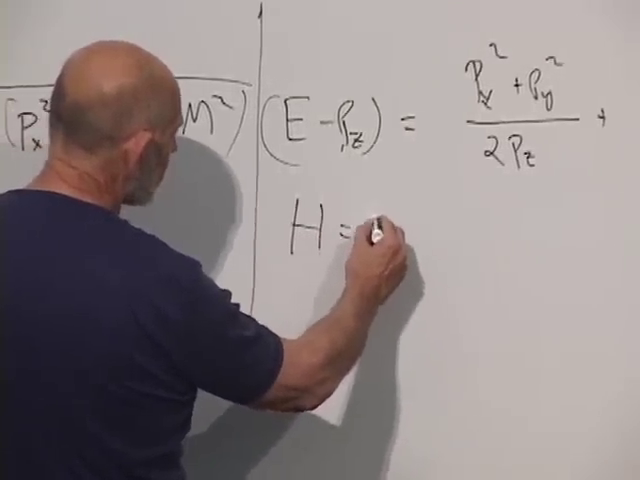
\includegraphics[width=\textwidth]{lecture_02_figure_02.png}\par\smallskip\footnotesize (a) Các biên dạng với đầu mút bị ghim và đầu mút phẳng.\end{minipage}\hfill
  \begin{minipage}[t]{0.48\textwidth}\centering
    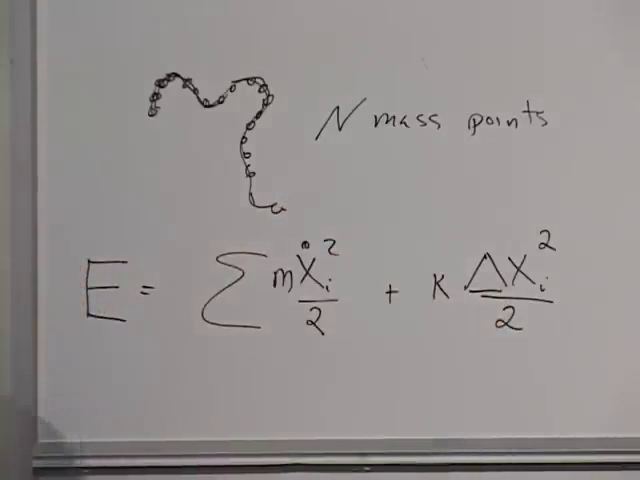
\includegraphics[width=\textwidth]{lecture_02_figure_03.png}\par\smallskip\footnotesize (b) Các vòng nhẹ trượt trên các cọc thẳng đứng.\end{minipage}\caption{Điều kiện biên dưới dạng hình dạng và dưới dạng cơ học. Cấu hình vòng trượt cho một đầu mút tự do một chuyển động ngang được xác định rõ ràng.}\lectureframe{00:08:50 and 00:12:15}\label{fig:l02-boundaries-board}\end{figure}

\begin{figure}[H]\centering
  \begin{adjustbox}{max width=\linewidth}\begin{tikzpicture}[>=Latex,thick,scale=0.92]
    \begin{scope}
      \draw[->] (0,0) -- (4.4,0) node[right] {\(\sigma\)};
      \draw[->] (0,-1.25) -- (0,1.35) node[above] {\(x\)};
      \draw[blue!70!black]
        (0,0) .. controls (0.8,1.1) and (1.4,1.0) .. (2.0,0)
        .. controls (2.7,-1.0) and (3.4,-0.8) .. (4.1,0);
      \fill (0,0) circle (0.06);
      \fill (4.1,0) circle (0.06);
      \node at (2.05,-1.65) {Dirichlet: \(x=0\)};
    \end{scope}
    \begin{scope}[xshift=5.8cm]
      \draw[->] (0,0) -- (4.4,0) node[right] {\(\sigma\)};
      \draw[->] (0,-1.25) -- (0,1.35) node[above] {\(x\)};
      \draw[orange!85!black]
        (0,0.65) .. controls (0.8,0.65) and (1.1,-0.9) .. (2.0,-0.9)
        .. controls (2.9,-0.9) and (3.2,0.55) .. (4.1,0.55);
      \draw[orange!85!black] (0,0.65) -- (0.45,0.65);
      \draw[orange!85!black] (3.65,0.55) -- (4.1,0.55);
      \node at (2.05,-1.65) {Neumann: \(\partial_\sigma x=0\)};
    \end{scope}
  \end{tikzpicture}\end{adjustbox}\caption{Giá trị được cố định đối với dữ liệu Dirichlet; độ dốc được cố định đối với dữ liệu Neumann.}\label{fig:l02-boundaries-redraw}\end{figure}

\begin{classroomqa}\audiencequestion{Một ống đàn organ hở hay kín có cho một ví dụ rõ ràng về một trong các điều kiện biên này không?\lecturetimestamp{00:09:19}}\lecturerresponse{Có thể, nhưng trước hết phải nói rõ đang khai triển biến âm học nào. Nhiễu loạn áp suất và độ dời dọc tuân theo những điều kiện lý tưởng hóa bổ sung lẫn nhau tại một đầu hở. Thay vì giải quyết câu hỏi bên lề ấy ngay trên bảng, hãy dùng mô hình vòng trượt: các vòng gần như không khối lượng có thể chuyển động thẳng đứng trên các cọc, nên các đầu mút của dây là tự do và bức tranh Neumann là trực tiếp.}\end{classroomqa}

\begin{classroomqa}\audiencequestion{Đồ thị có thể dựng đứng và chứa một bước nhảy đột ngột không?\lecturetimestamp{00:09:53}}\lecturerresponse{Phân tích Fourier cho phép những bước nhảy cô lập trong một hàm liên tục từng khúc. Một dây vật lý thì bị ràng buộc chặt hơn. Một bước nhảy làm các điểm lân cận mất liên thông và khiến đạo hàm theo không gian \(\partial_\sigma x\) trở nên kỳ dị trong năng lượng liên tục sẽ được suy ra bên dưới. Vì vậy ta chỉ giới hạn sự chú ý vào các biên dạng liên tục và khả vi.}\end{classroomqa}

\begin{classroomqa}\audiencequestion{Tại sao đầu hở của một ống, hay bất kỳ đầu tự do nào, lại phải thỏa một điều kiện biên?\lecturetimestamp{00:11:14}}\lecturerresponse{Ví dụ âm học phụ thuộc vào trường được chọn và đã được để ngỏ trong phần thảo luận. Ví dụ cơ học thì không. Một vòng rất nhẹ được tự do trượt nhưng vẫn gắn với đoạn dây cuối cùng. Ta sẽ suy ra điều kiện của nó từ định luật Newton thay vì giả sử trước: gia tốc hữu hạn ở đầu mút buộc độ dốc phải triệt tiêu.}\end{classroomqa}

\subsection{Các cơ sở Fourier}

Một khi kiểu điều kiện ở đầu mút đã được cố định, cơ sở Fourier tương ứng cũng được cố định. Trên \(0\leq\sigma\leq\pi\),

\begin{align}
  x_D(\sigma)
  &=
  \sum_{n=1}^{\infty}x_n\sin(n\sigma),
  \label{eq:l02-dirichlet-series}\\
  x_N(\sigma)
  &=
  \sum_{n=0}^{\infty}x_n\cos(n\sigma).
  \label{eq:l02-neumann-series}
\end{align}

Mọi hàm sin trong \eqref{eq:l02-dirichlet-series} đều triệt tiêu tại cả hai đầu mút. Mọi hàm cos trong \eqref{eq:l02-neumann-series} đều có đạo hàm ở đầu mút bằng không. Các cận dưới khác nhau là có lý do: \(\sin(0\sigma)=0\) không đóng góp gì, còn \(\cos(0\sigma)=1\) là mode hằng, hay mode không. Nó ghi lại giá trị trung bình của một hàm Neumann.

\begin{figure}[H]\centering
  \begin{minipage}[t]{0.48\textwidth}\centering
    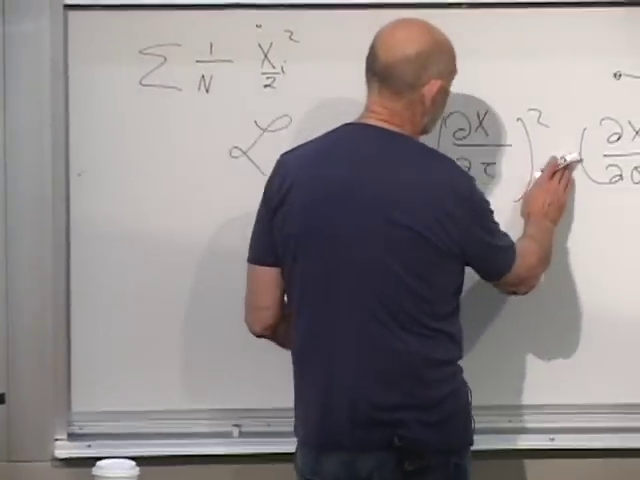
\includegraphics[width=\textwidth]{lecture_02_figure_04.png}\par\smallskip\footnotesize (a) Khai triển sin và cos.\end{minipage}\hfill
  \begin{minipage}[t]{0.48\textwidth}\centering
    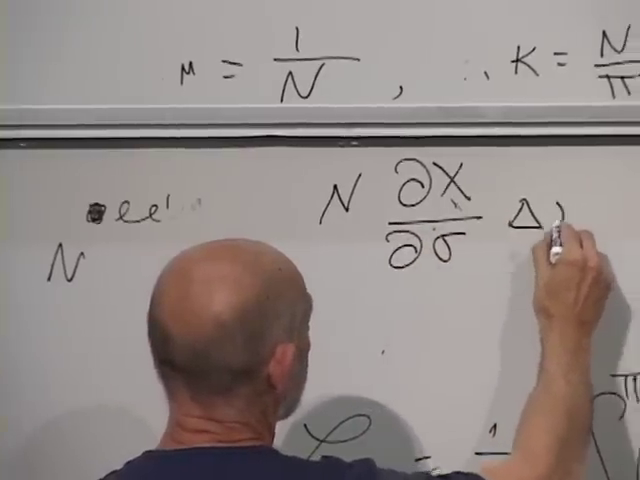
\includegraphics[width=\textwidth]{lecture_02_figure_05.png}\par\smallskip\footnotesize (b) Tính trực giao và mode hằng ngoại lệ.\end{minipage}\caption{Các tính chất Fourier sẽ được dùng về sau để chéo hóa dây.}\lectureframe{00:16:15 and 00:20:30}\label{fig:l02-fourier-board}\end{figure}

Phép lấy đạo hàm hoán đổi hai lớp này:

\begin{equation}
  \begin{aligned}
    \partial_\sigma\sin(n\sigma)&=n\cos(n\sigma),\\
    \partial_\sigma\cos(n\sigma)&=-n\sin(n\sigma).
  \end{aligned}
  \label{eq:l02-basis-derivatives}
\end{equation}

Do đó, đạo hàm của một chuỗi Dirichlet có tính chất Neumann, còn đạo hàm của một chuỗi Neumann có tính chất Dirichlet. Khi ấy tính trực giao khử các hạng chéo giữa những mode khác nhau:

\begin{align}
  \int_0^\pi\cos(n\sigma)\cos(m\sigma)\,d\sigma
  &=
  \frac{\pi}{2}\delta_{nm},
  && n,m\geq1,
  \label{eq:l02-cos-orthogonality}\\
  \int_0^\pi\sin(n\sigma)\sin(m\sigma)\,d\sigma
  &=
  \frac{\pi}{2}\delta_{nm},
  && n,m\geq1,
  \label{eq:l02-sin-orthogonality}\\
  \int_0^\pi 1\,d\sigma&=\pi .
  \label{eq:l02-zero-norm}
\end{align}

Dòng cuối cùng là chuẩn cos ngoại lệ ứng với \(n=m=0\). Một hằng số không được chuẩn hóa như một điều hòa khác không, và hệ số 2 ấy sẽ phân biệt mode khối tâm của dây với các mode nội tại của nó.

\subsection{Một công thức dao động tử cần nhớ}

Sau khi đổi tỷ lệ một tọa độ sao cho khối lượng cơ học của nó bằng một, một dao động tử theo định luật Hooke có

\begin{align}
  E_{\mathrm{osc}}
  &=
  \frac12\dot q^{\,2}
  +\frac12\omega^2q^2,
  \label{eq:l02-oscillator-energy}\\
  L_{\mathrm{osc}}
  &=
  \frac12\dot q^{\,2}
  -\frac12\omega^2q^2.
  \label{eq:l02-oscillator-lagrangian}
\end{align}

\begin{figure}[H]\centering
  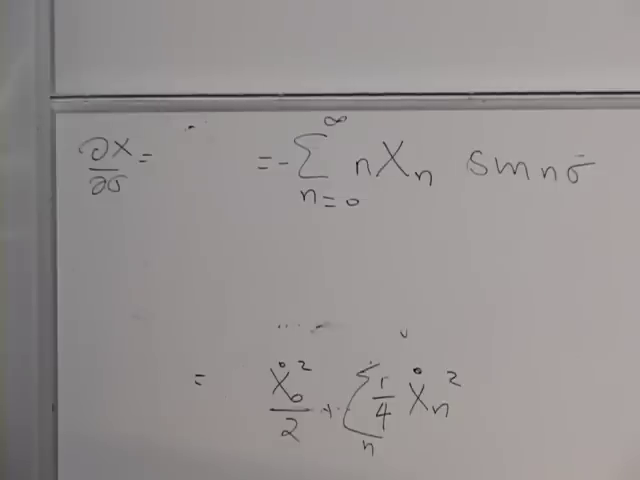
\includegraphics[width=0.68\textwidth]{lecture_02_figure_06.png}\caption{Năng lượng của dao động tử, được viết sao cho hệ số của \(q^2\) lập tức cho biết \(\omega^2\).}\lectureframe{00:24:00}\label{fig:l02-oscillator-board}\end{figure}

Về mặt cổ điển, \(\omega=\sqrt{\kappa/m}\); phép đổi tỷ lệ tọa độ đã đặt \(m=1\). Về mặt lượng tử,

\begin{equation}
  E_Q=\hbar\omega\left(Q+\frac12\right),
  \qquad Q=0,1,2,\ldots .
  \label{eq:l02-oscillator-spectrum}
\end{equation}

Khi xét khoảng cách mức, ta có thể trừ đi hạng trạng thái cơ bản chung và nói rằng mỗi lượng tử tốn \(\hbar\omega\). Ban đầu phép tính cho dây sẽ làm đúng như vậy và hoãn việc xử lý tổng năng lượng điểm không lại.

\begin{classroomqa}
\audiencequestion{Tần số của dao động tử được đọc ra từ công thức năng lượng như thế nào?\lecturetimestamp{00:23:21}}
\lecturerresponse{Trước khi đổi tỷ lệ, nó là \(\omega=\sqrt{\kappa/m}\). Khi khối lượng bằng một, hạng thế năng là \(\frac12\omega^2q^2\), nên hệ số bậc hai của nó chính là bình phương của tần số.}
\end{classroomqa}

\section{Điều gì làm cho một hệ hợp thành trở thành một hạt?}

Một dây có độ trải rộng và sẽ được mô hình hóa bằng nhiều phần tử liên kết với nhau. Vậy theo nghĩa nào một trong các trạng thái lượng tử của nó vẫn có thể là một hạt? Tính điểm không thể là tiêu chuẩn quyết định. Proton và neutron là những hệ hợp thành. Electron và photon đều đi kèm với một lớp bao bọc của trường lượng tử, dù chưa phân giải được cấu trúc con nội tại nào. Một điểm hình học cổ điển không có gì bao quanh không phải là hình ảnh đúng của một kích thích lượng tử.

Khối lượng và vị trí khối tâm cũng không đủ. Một hộp khí kín có cả hai. Một tách cà phê cũng có cả hai. Ta thường không gọi cái nào trong hai thứ ấy là một hạt. Tính không thể chia cắt cũng thất bại, vì proton là khả phân, và spin không phân biệt các hạt vi mô với các vật thể vĩ mô.

Tiêu chuẩn hữu ích là sự cô lập phổ. Đặt năng lượng nghỉ trên một trục đứng và hỏi cần bao nhiêu năng lượng để đạt tới một trạng thái nội tại khác. Electron không có một tháp các kích thích electron nằm ngay phía trên mà thí nghiệm có thể tiếp cận. Proton thì có các cộng hưởng, nhưng những cộng hưởng đầu tiên cần vài trăm MeV, một phần đáng kể của khối lượng proton. Các trạng thái đó tách nhau đủ xa để có thể nhận diện riêng rẽ.

Một tách cà phê thì ngược lại. Người ta có thể thêm một lượng năng lượng nhỏ tùy ý vào một mode âm thanh bước sóng dài, khẽ tác động lên một phân tử, hoặc tạo ra một phonon. Có rất nhiều trạng thái chen chúc trong một khoảng rất nhỏ. Ở các thang đo phòng thí nghiệm, chúng tạo thành một liên tục. Đây là sự phân biệt thực dụng giữa một hạt và \emph{một khối nhão}.

\begin{figure}[H]\centering
  \includegraphics[width=0.58\textwidth]{lecture_02_figure_07.png}\caption{Trục năng lượng thẳng đứng trên bảng khi so sánh một mức hạt cô lập với các kích thích dày đặc của vật chất thông thường.}\lectureframe{00:31:10}\label{fig:l02-spectrum-board}\end{figure}

\begin{figure}[H]\centering
  \begin{adjustbox}{max width=\linewidth}\begin{tikzpicture}[>=Latex,thick]
    \begin{scope}
      \draw[->] (0,0) -- (0,4.8) node[above] {energy};
      \draw[blue!70!black,line width=1.2pt] (-1.0,0.65) -- (1.0,0.65);
      \draw[blue!70!black,line width=1.2pt] (-1.0,3.65) -- (1.0,3.65);
      \node[right] at (1.05,0.65) {ground state};
      \node[right] at (1.05,3.65) {first internal excitation};
      \draw[<->] (0.65,0.75) -- (0.65,3.55)
        node[midway,right] {large gap};
      \node at (0,-0.55) {particle-like};
    \end{scope}
    \begin{scope}[xshift=7.0cm]
      \draw[->] (0,0) -- (0,4.8) node[above] {energy};
      \foreach \y in {0.55,0.69,0.82,0.94,1.05,1.15,1.24,1.32,1.39,1.45,
        1.51,1.57,1.63,1.70,1.78,1.87,1.97,2.09,2.22,2.36,2.51,2.67,2.84,
        3.02,3.21,3.41,3.62,3.84,4.07}
        \draw[orange!85!black] (-0.95,\y) -- (0.95,\y);
      \node[right] at (1.05,2.25) {dense phonon and internal states};
      \node at (0,-0.55) {macroscopic matter};
    \end{scope}
  \end{tikzpicture}\end{adjustbox}\caption{Sự cô lập phổ, chứ không phải tính điểm theo nghĩa đen, là tiêu chuẩn thao tác về hạt được dùng trong bài giảng.}\label{fig:l02-particle-redraw}\end{figure}

Tiêu chuẩn này biến câu hỏi triết học thành một phép tính. Hãy lượng tử hóa dây, tìm các mức năng lượng nội tại của nó, rồi xem xét khoảng cách giữa chúng. Nếu trạng thái kích thích đầu tiên của dây nằm gần thang Planck trong khi trạng thái cơ bản quan sát được là nhẹ, thì khe đó vượt quá năng lượng của các máy gia tốc hiện nay hơn 20 bậc độ lớn. Khi ấy dây hành xử như một hạt cơ bản trong toàn bộ miền có thể tiếp cận.

\begin{classroomqa}\audiencequestion{Hành vi hạt có chỉ đơn thuần là vấn đề thang quan sát không? Nếu ta phóng to đủ mức, các mức có thôi tách biệt nữa không?\lecturetimestamp{00:33:33}}\lecturerresponse{Việc nhìn đủ kỹ có thể cho thấy một đối tượng có nhiều thành phần cấu tạo, nhưng nó không xóa phổ đi. So sánh thích hợp là giữa độ phân giải năng lượng của thí nghiệm và khe tới kích thích nội tại đầu tiên. Một đối tượng hợp thành vẫn có thể mang tính hạt khi khe đó là rất lớn.}\end{classroomqa}

\begin{classroomqa}\audiencequestion{Tại sao một dây đàn vĩ cầm thông thường lại không phải là một hạt?\lecturetimestamp{00:34:37}}\lecturerresponse{Một lượng tử dao động mang năng lượng nhỏ đến mức không thể đo được so với năng lượng nghỉ của sợi dây vĩ mô. Vì vậy, nhiều trạng thái lượng tử chen vừa vào một khoảng tương đối rất nhỏ. Nó thuộc về phía dày đặc của phép so sánh phổ, chứ không phải phía cô lập.}\end{classroomqa}

\begin{classroomqa}\audiencequestion{Photon và electron có phải là hạt điểm không, nếu xung quanh chúng có các thăng giáng ảo của trường lượng tử?\lecturetimestamp{00:35:40}}\lecturerresponse{Từ cổ điển \emph{điểm} đang phải gánh quá nhiều ý nghĩa. Electron và photon vật lý là các kích thích trường đã được hiệu chỉnh, nhưng thực nghiệm chưa tìm thấy ở bên nào cấu trúc thành phần nội tại hay nhân tử dạng hữu hạn. Điều quan trọng đối với lập luận hiện tại là không bên nào có một tháp dày đặc các trạng thái nội tại gần suy biến.\editorialnote{Bài giảng liên hệ mômen từ dị thường của electron với một độ mờ lượng tử có thể đo được. Theo thuật ngữ hiện đại, mômen dị thường là một hiệu ứng hiệu chỉnh bức xạ, chứ không phải bằng chứng về một bán kính electron hữu hạn đã được phân giải. Theo quy ước, dạng điểm có nghĩa là chưa phát hiện được cấu trúc con nội tại hay nhân tử dạng nào xuống tới thang đã được kiểm nghiệm.}}\end{classroomqa}

\begin{classroomqa}\audiencequestion{Kích thước của photon có phụ thuộc vào tần số của nó không?\lecturetimestamp{00:36:49}}\lecturerresponse{Bước sóng của nó thì chắc chắn có phụ thuộc. Điều đó khác với một kích thước thành phần nội tại. Việc thay đổi tần số làm thay đổi gói sóng và bước sóng, chứ không phải một bán kính nội tại của photon đã được phân giải.}\end{classroomqa}

\section{Cơ học ngang chính xác ở xung lượng lớn}

Bây giờ ta quay lại khó khăn tương đối tính. Một cây gậy quay nhanh không thể được xử lý phi tương đối tính chỉ bằng cách đặt khối tâm của nó đứng yên. Các đầu của nó vẫn chuyển động tương đối tính đối với nhau. Xấp xỉ phi tương đối tính thất bại vì chuyển động tương đối nội bộ.

Tuy nhiên, có một giới hạn khác. Chọn một trục \(z\) và thực hiện một phép boost cho toàn bộ hệ tới một xung lượng dọc dương rất lớn \(P_z\). Giữ xung lượng ngang của nó

\begin{equation}
  p_\perp^2=p_x^2+p_y^2
\end{equation}

hữu hạn. Khi đó phép chiếu theo phương ngang có dạng Hamilton phi tương đối tính một cách chính xác trong giới hạn \(P_z\to\infty\), ngay cả khi chuyển động nội bộ trước phép boost là tương đối tính.

\begin{classroomqa}
\audiencequestion{Động lượng vô hạn có nghĩa là hệ có khối lượng thực sự đạt tới tốc độ ánh sáng không?\lecturetimestamp{00:40:43}}
\lecturerresponse{Không có phép boost hữu hạn nào đạt tới tốc độ ấy. Người ta xây dựng các đại lượng có giới hạn xác định khi \(P_z\) trở nên lớn tùy ý. Cụm từ này chỉ một quy trình lấy giới hạn, không phải một trạng thái vật lý hữu hạn với \(v=c\).}
\end{classroomqa}

\begin{classroomqa}
\audiencequestion{Phải chọn trục nào, và điều gì xảy ra nếu vật quay quanh hoặc ngang qua trục đó?\lecturetimestamp{00:41:14}}
\lecturerresponse{Có thể chọn bất kỳ trục nào và boost toàn bộ hệ dọc theo trục ấy. Điều còn lại dưới dạng cơ học tường minh là hình chiếu lên mặt phẳng vuông góc. Một thanh quay có thể trông bị co ngắn lại hoặc quét qua mặt phẳng đó, nhưng hình chiếu ngang của nó có dạng phi tương đối tính.}
\end{classroomqa}

Dây có thêm một tính chất khiến biểu diễn này đặc biệt mạnh. Trong chuẩn light-front, các tọa độ nội tại dọc của nó không phải là những dao động tử độc lập. Các ràng buộc xác định chúng từ chuyển động ngang. Vì vậy, chỉ cần biết cấu hình ngang của dây là đủ để tái dựng các bậc tự do vật lý.

\begin{classroomqa}
\audiencequestion{Việc không có một tọa độ dọc độc lập có nghĩa là dây chỉ đơn thuần bị kẹt trong một lớp mỏng hay không?\lecturetimestamp{00:42:26}}
\lecturerresponse{Sự co Lorentz quả thật làm cho độ dài dọc của nó nhỏ trong hệ quy chiếu được boost, nhưng phát biểu ở đây còn mạnh hơn. Mọi chuyển động dọc còn lại đều bị chuyển động ngang ràng buộc; không thể được chỉ định độc lập.}
\end{classroomqa}

\begin{classroomqa}
\audiencequestion{Sự quy giản này về dữ liệu ngang có liên quan đến nguyên lý toàn ảnh không?\lecturetimestamp{00:43:12}}
\lecturerresponse{Nó liên hệ chặt chẽ với mạch tư duy đã dẫn tới các ý tưởng toàn ảnh, mặc dù theo đuổi mối liên hệ ấy sẽ đưa ta ra khỏi phép tính hiện tại. Ở đây nó chỉ dùng để biện minh cho việc làm việc với cấu hình ngang của dây.}
\end{classroomqa}

\subsection{Trừ phần do boost và đổi thang thời gian}

Gọi \(M\) là khối lượng bất biến của toàn hệ, bao gồm khối lượng các thành phần, động năng và năng lượng liên kết. Trong đơn vị \(c=1\),

\begin{equation}
  E=\sqrt{P_z^2+p_\perp^2+M^2}.
  \label{eq:l02-relativistic-energy}
\end{equation}

Với \(P_z\) lớn hơn nhiều so với \(p_\perp\) và \(M\),

\begin{equation}
  E
  =
  P_z+\frac{p_\perp^2+M^2}{2P_z}
  +O(P_z^{-3}).
  \label{eq:l02-large-pz}
\end{equation}

\begin{figure}[H]
  \centering
  \includegraphics[width=0.76\textwidth]{lecture_02_figure_08.png}
  \caption{Khai triển đầy đủ theo large-\(P_z\), trong đó động lượng ngang và khối lượng bất biến được giữ lại.}
  \lectureframe{00:47:30}
  \label{fig:l02-large-pz-board}
\end{figure}

Hạng dẫn đầu rất lớn, nhưng nó không mang thông tin nào về trạng thái nội. Trong một quá trình bảo toàn \(P_z\), chẳng hạn một nguyên tử được boost chuyển giữa các mức nội mà không thay đổi tổng động lượng dọc của nó, hạng ấy triệt tiêu khỏi mọi hiệu năng lượng. Vì vậy ta khảo sát

\begin{equation}
  E-P_z=\frac{p_\perp^2+M^2}{2P_z}+O(P_z^{-3}).
  \label{eq:l02-residual-energy}
\end{equation}

Mẫu số có một ý nghĩa vật lý. Vì Hamiltonian sinh ra sự tiến hóa theo thời gian, năng lượng dư nhỏ cho thấy sự tiến hóa nội có vẻ chậm trong thời gian phòng thí nghiệm. Đó là giãn thời gian. Để giữ lại chuyển động nội, ta đưa vào một tham số tiến hóa đã đổi thang \(\tau\), hoặc tương đương nhân Hamiltonian dư với \(P_z\):

\begin{equation}
  H_\perp
  \equiv
  \lim_{P_z\to\infty}P_z(E-P_z)
  =
  \frac12p_\perp^2+\frac12M^2.
  \label{eq:l02-transverse-hamiltonian}
\end{equation}

\begin{figure}[H]
  \centering
  \begin{minipage}[t]{0.48\textwidth}
    \centering
    \includegraphics[width=\textwidth]{lecture_02_figure_09.png}
    \par\smallskip\footnotesize (a) \(H=i\partial_t\) và sự tiến hóa nội bị làm chậm.
  \end{minipage}\hfill
  \begin{minipage}[t]{0.48\textwidth}
    \centering
    \includegraphics[width=\textwidth]{lecture_02_figure_10.png}
    \par\smallskip\footnotesize (b) Hamiltonian ngang hữu hạn sau khi đổi thang thời gian.
  \end{minipage}
  \caption{Từ năng lượng dư đã bị giãn thời gian đến một Hamiltonian hai chiều hữu hạn.}
  \lectureframe{00:49:20 and 00:52:40}
  \label{fig:l02-lightfront-board}
\end{figure}

Đây chính xác là dạng của một hạt khối lượng đơn vị chuyển động trong hai chiều: động năng \(p_\perp^2/2\) cộng với một năng lượng nội \(M^2/2\). Điểm khác thường là bình phương. Trong mô tả này, đại lượng đóng vai trò năng lượng nghỉ hay năng lượng liên kết tỉ lệ với bình phương khối lượng bất biến.\editorialnote{Với các biến light-front thông thường \(P^\pm=(E\pm P_z)/\sqrt2\), hệ thức vỏ khối lượng chính xác là \(2P^+P^-=p_\perp^2+M^2\). Phương trình \eqref{eq:l02-transverse-hamiltonian} là cách chuẩn hóa large-\(P_z\) của bài giảng cho cùng một hệ thức bất biến.}

\begin{classroomqa}
\audiencequestion{Các động lượng dọc của từng phần riêng lẻ trong một hệ hợp thành đã đi đâu?\lecturetimestamp{00:51:30}}
\lecturerresponse{Đối với một vật hợp thành tổng quát, ta phải giữ lại các tỉ phần của tổng \(P_z\) do các thành phần của nó mang. Công thức trên dùng tổng động lượng của khối tâm. Lý thuyết dây là đặc biệt vì các ràng buộc của nó xác định chuyển động dọc tương đối từ các bậc tự do ngang, nên không cần thêm một dao động tử dọc độc lập nào.}
\end{classroomqa}

\section{Một dây mở rời rạc}

Dây được boost giờ đây tường minh chỉ chuyển động trong mặt phẳng ngang. Gọi hai tọa độ của nó là \(X\) và \(Y\), và trước hết xấp xỉ nó bằng \(N\) chất điểm được nối với nhau bởi \(N-1\) lò xo. Nếu \(\mu\) là khối lượng tương tự của mỗi điểm và \(k\) là hằng số đàn hồi giữa các láng giềng gần, thì năng lượng là

\begin{equation}
  E_N
  =
  \sum_i
  \left[
    \frac{\mu}{2}
    \left(\dot X_i^2+\dot Y_i^2\right)
    +
    \frac{k}{2}
    \left((\Delta X_i)^2+(\Delta Y_i)^2\right)
  \right].
  \label{eq:l02-discrete-energy}
\end{equation}

Mỗi hạng \(X\) đều có một hạng \(Y\) giống hệt, vì mặt phẳng ngang có hai phương. Chỉ số \(i\) gắn nhãn một điểm dọc theo chuỗi; nó không phải là một tọa độ không gian.

\begin{figure}[H]
  \centering
  \begin{minipage}[t]{0.48\textwidth}
    \centering
    \includegraphics[width=\textwidth]{lecture_02_figure_11.png}
    \par\smallskip\footnotesize (a) Chuỗi hạt và năng lượng rời rạc của nó.
  \end{minipage}\hfill
  \begin{minipage}[t]{0.48\textwidth}
    \centering
    \includegraphics[width=\textwidth]{lecture_02_figure_12.png}
    \par\smallskip\footnotesize (b) Quy luật tỉ lệ large-\(N\) của \(\mu\) và \(k\).
  \end{minipage}
  \caption{Dây mở được điều chuẩn trước khi lấy giới hạn liên tục.}
  \lectureframe{00:57:42 and 01:02:40}
  \label{fig:l02-chain-board}
\end{figure}

\begin{figure}[H]
  \centering
  \begin{adjustbox}{max width=\linewidth}
  \begin{tikzpicture}[>=Latex,thick]
    \foreach \i in {0,...,8} {
      \coordinate (p\i) at ({1.05*\i},{0.30*sin(55*\i)});
      \filldraw[white] (p\i) circle (0.10);
      \draw (p\i) circle (0.10);
    }
    \foreach \i in {0,...,7} {
      \pgfmathtruncatemacro{\j}{\i+1}
      \draw[decorate,decoration={zigzag,segment length=4pt,amplitude=2pt}]
        (p\i) -- (p\j);
    }
    \node[above=0.35cm of p0] {\(i=0\)};
    \node[above=0.35cm of p8] {\(i=N-1\)};
    \draw[<->] (0,-1.15) -- (8.4,-1.15)
      node[midway,below] {\(0\leq\sigma\leq\pi\)};
    \node at (4.2,1.25)
      {\(\mu=1/N,\quad k=N/\pi^2,\quad\Delta\sigma=\pi/N\)};
  \end{tikzpicture}
  \end{adjustbox}
  \caption{Một hình ảnh điều chuẩn rõ ràng. Khi chuỗi được tinh luyện hơn, các điểm trở nên nhẹ hơn còn các lò xo vi mô trở nên cứng hơn.}
  \label{fig:l02-chain-redraw}
\end{figure}

Tham số \(\sigma\) gắn nhãn vị trí dọc theo chuỗi. Việc chọn \(0\leq\sigma\leq\pi\) là một quy ước, không phải một phép đo độ dài vật lý. Nó nhắc ta rằng dây có hai đầu mút. Sau này, một dây kín sẽ được gắn nhãn tuần hoàn trên \(0\leq\sigma<2\pi\).

Giới hạn liên tục phải giữ cho cơ học tập thể là hữu hạn. Nếu giữ cố định khối lượng mỗi hạt, tổng khối lượng tương tự sẽ phân kỳ, nên hãy chọn

\begin{equation}
  \mu=\frac{1}{N}.
  \label{eq:l02-mu-scaling}
\end{equation}

Khi đó \(N\mu=1\). Đây không phải là khối lượng nghỉ tương đối tính \(M\); nó là hệ số quán tính trong mô hình tương tự ngang.

Các lò xo mắc nối tiếp trở nên mềm hơn khi số lượng của chúng tăng lên. Để bảo toàn một độ cứng hữu hạn cho toàn chuỗi, mỗi lò xo vi mô phải trở nên cứng hơn:

\begin{equation}
  k=\frac{N}{\pi^2}
  =\frac{1}{\pi\,\Delta\sigma}.
  \label{eq:l02-k-scaling}
\end{equation}

Chỉ \(k\propto N\) là thiết yếu. Hệ số \(\pi^2\) là một chuẩn hóa được chọn để loại bỏ các hệ số \(\pi\) lạc lõng khỏi các công thức liên tục.

\begin{classroomqa}
\audiencequestion{Liệu \(\mu\) có phải là khối lượng nghỉ vật lý của mỗi điểm trên dây không?\lecturetimestamp{01:10:34}}
\lecturerresponse{Không. Nó là khối lượng tương tự phi tương đối tính xuất hiện trong chuỗi ngang. Gọi nó là \(M\) sẽ gây nhầm lẫn với khối lượng nghỉ bất biến của toàn trạng thái dây tương đối tính. Vai trò duy nhất của nó ở đây là tạo ra quán tính liên tục đúng.}
\end{classroomqa}

\section{Hệ sóng liên tục}

Hãy áp dụng các quy tắc đã chuẩn bị ở phần đầu. Vì \(1/N=\Delta\sigma/\pi\),

\begin{align}
  \sum_i\frac{\mu}{2}\dot X_i^2
  &=
  \frac{1}{2\pi}
  \sum_i\dot X_i^2\,\Delta\sigma
  \longrightarrow
  \frac{1}{2\pi}
  \int_0^\pi
  \left(\partial_\tau X\right)^2d\sigma ,
  \label{eq:l02-kinetic-limit}\\
  \sum_i\frac{k}{2}(\Delta X_i)^2
  &\longrightarrow
  \frac{1}{2\pi}
  \int_0^\pi
  \left(\partial_\sigma X\right)^2d\sigma .
  \label{eq:l02-potential-limit}
\end{align}

Đối với dòng thứ hai, dùng \(\Delta X_i=\partial_\sigma X\,\Delta\sigma\) cùng với \(k=1/(\pi\Delta\sigma)\). Phép tính tương tự cũng áp dụng cho \(Y\).

\begin{figure}[H]
  \centering
  \begin{minipage}[t]{0.48\textwidth}
    \centering
    \includegraphics[width=\textwidth]{lecture_02_figure_13.png}
    \par\smallskip\footnotesize (a) Các phép thay tổng bằng tích phân và sai phân bằng đạo hàm.
  \end{minipage}\hfill
  \begin{minipage}[t]{0.48\textwidth}
    \centering
    \includegraphics[width=\textwidth]{lecture_02_figure_14.png}
    \par\smallskip\footnotesize (b) Biểu thức năng lượng liên tục hoàn chỉnh.
  \end{minipage}
  \caption{Chuỗi rời rạc trở thành một trường trên khoảng \(\sigma\).}
  \lectureframe{01:05:40 and 01:07:00}
  \label{fig:l02-continuum-board}
\end{figure}

Năng lượng và Lagrangian thu được là

\begin{align}
  E
  &=
  \frac{1}{2\pi}
  \int_0^\pi d\sigma\,
  \left[
    (\partial_\tau X)^2+(\partial_\tau Y)^2\right.\notag\\[-0.25em]
  &\hspace{6.5em}\left.
    +(\partial_\sigma X)^2+(\partial_\sigma Y)^2
  \right],
  \label{eq:l02-continuum-energy}\\
  L
  &=
  \frac{1}{2\pi}
  \int_0^\pi d\sigma\,
  \left[
    (\partial_\tau X)^2+(\partial_\tau Y)^2\right.\notag\\[-0.25em]
  &\hspace{6.5em}\left.
    -(\partial_\sigma X)^2-(\partial_\sigma Y)^2
  \right].
  \label{eq:l02-continuum-lagrangian}
\end{align}

\begin{figure}[H]
  \centering
  \includegraphics[width=0.78\textwidth]{lecture_02_figure_15.png}
  \caption{Lagrangian liên tục với các hạng động năng và kéo dãn mang dấu đối nhau.}
  \lectureframe{01:08:48}
  \label{fig:l02-lagrangian-board}
\end{figure}

Nếu ta đổi tên \(\sigma\) thành một tọa độ không gian thông thường và \(X\) thành một trường \(\phi\), thì đây là năng lượng và Lagrangian của một trường sóng một chiều. Lấy biến phân \eqref{eq:l02-continuum-lagrangian} cho

\begin{equation}
  \left(\partial_\tau^2-\partial_\sigma^2\right)X=0,
  \qquad
  \left(\partial_\tau^2-\partial_\sigma^2\right)Y=0.
  \label{eq:l02-wave-equation}
\end{equation}

Không có gì trong lập luận trước mắt buộc ta phải giải trực tiếp các phương trình này. Bức tranh hữu ích đơn giản là các sóng truyền sang trái và sang phải dọc theo dây và phản xạ tại các đầu mút. Phản xạ Dirichlet đảo dấu độ dời; phản xạ Neumann giữ nguyên dấu đó.

\begin{classroomqa}
\audiencequestion{Chính xác thì biến thời gian \(\tau\) là gì?\lecturetimestamp{01:08:54}}
\lecturerresponse{Đó là thời gian đã được đổi thang dùng để theo dõi chuyển động nội trong mô tả large-\(P_z\). Một chiếc đồng hồ được boost cùng hệ chạy chậm so với thời gian phòng thí nghiệm; \(\tau\) loại bỏ sự giãn ấy để các dao động nội giữ được một tốc độ hữu hạn. Đối với cơ học ngang này, có thể đơn giản coi nó là thời gian.\editorialnote{Bài giảng gọi \(\tau\) một cách không chặt chẽ là thời gian riêng. Đối với một dây mở rộng, tham số tiến hóa light-front chính xác là một thời gian đã đổi thang sau khi cố định chuẩn, chứ không phải một thời gian riêng bất biến duy nhất được mọi điểm cùng chia sẻ. Luận điểm về giãn thời gian được nhắm đến không thay đổi.}}
\end{classroomqa}

Khi khối tâm đứng yên trong mặt phẳng ngang, phần nội của \eqref{eq:l02-continuum-energy}, theo chuẩn hóa của \eqref{eq:l02-transverse-hamiltonian}, tỉ lệ với \(M^2\). Đó là lý do lượng tử hóa hệ sóng có vẻ thông thường này sẽ làm lộ ra phổ khối lượng tương đối tính.

\begin{classroomqa}
\audiencequestion{\(P_z(E-P_z)\) có tên gọi nào không?\lecturetimestamp{01:11:00}}
\lecturerresponse{Nó thường được gọi là năng lượng light-cone hay light-front. Light front mô tả thích hợp hơn siêu phẳng không được dùng làm mặt tiến hóa; thuật ngữ truyền thống không quan trọng đối với phép tính.}
\end{classroomqa}

\begin{classroomqa}
\audiencequestion{Từ cone ở đây có chỉ nón ánh sáng không-thời gian quen thuộc, và Dirac có đưa ra thuật ngữ này không?\lecturetimestamp{01:11:17}}
\lecturerresponse{Cách dựng bằng tọa độ null có thể được vẽ với các trục 45 độ, nhưng mặt tiến hóa ở đây là một light front chứ không phải toàn bộ nón đang nở ra. Dirac đã phát triển các dạng tương ứng của động lực học tương đối tính; câu hỏi lịch sử về tên gọi được để ngỏ và không ảnh hưởng đến các phương trình.}
\end{classroomqa}

\section{Vì sao đầu mút tự do là Neumann}

Giờ đây ta có thể suy ra thay vì chỉ giả định điều kiện ở đầu mút. Định luật Newton là hợp lệ vì cơ học ngang sau boost có đúng dạng phi tương đối tính. Một điểm khối lượng ở bên trong bị kéo bởi các lò xo ở cả hai phía. Điểm cuối cùng chỉ bị kéo bởi lò xo nối nó với điểm láng giềng.

\begin{classroomqa}
\audiencequestion{Tại sao ta được phép dùng định luật Newton trong khi đang bàn về một dây tương đối tính?\lecturetimestamp{01:14:52}}
\lecturerresponse{Ta không áp dụng cơ học Newton cho chuyển động không-thời gian đầy đủ, chưa boost. Ta áp dụng nó cho các biến ngang trong mô tả động lượng vô hạn, mà Hamiltonian của nó có đúng dạng phi tương đối tính.}
\end{classroomqa}

Tại đầu mút phải, định luật Hooke cho, tùy theo quy ước hướng,

\begin{equation}
  F_{\mathrm{end}}
  =
  -k\,\Delta X
  =
  -\frac{1}{\pi\Delta\sigma}
   \left(\partial_\sigma X\,\Delta\sigma\right)
  =
  -\frac{1}{\pi}\partial_\sigma X .
  \label{eq:l02-endpoint-force}
\end{equation}

\begin{figure}[H]
  \centering
  \begin{minipage}[t]{0.48\textwidth}
    \centering
    \includegraphics[width=\textwidth]{lecture_02_figure_16.png}
    \par\smallskip\footnotesize (a) Lực ở đầu mút tỉ lệ với độ dốc cục bộ.
  \end{minipage}\hfill
  \begin{minipage}[t]{0.48\textwidth}
    \centering
    \includegraphics[width=\textwidth]{lecture_02_figure_17.png}
    \par\smallskip\footnotesize (b) Điều kiện gia tốc hữu hạn.
  \end{minipage}
  \caption{Phép suy ra điều kiện biên đầu tự do bằng định luật Newton.}
  \lectureframe{01:18:20 and 01:20:10}
  \label{fig:l02-neumann-board}
\end{figure}

Phương trình Newton cho điểm cuối là

\begin{equation}
  \mu\,\partial_\tau^2X=F_{\mathrm{end}},
  \qquad
  \mu=\frac1N=\frac{\Delta\sigma}{\pi}.
  \label{eq:l02-endpoint-newton}
\end{equation}

Kết hợp \eqref{eq:l02-endpoint-force} và \eqref{eq:l02-endpoint-newton},

\begin{equation}
  \partial_\sigma X
  =
  -\Delta\sigma\,\partial_\tau^2X
  \quad\text{at the right endpoint},
  \label{eq:l02-endpoint-scaling}
\end{equation}

với dấu của lực đảo ngược ở đầu mút trái. Nếu \(\partial_\sigma X\) tiến tới một hằng số khác không trong khi \(\Delta\sigma\to0\), thì gia tốc ở đầu mút sẽ phân kỳ như \(N\). Vì vậy, một giới hạn liên tục hợp lý với gia tốc hữu hạn đòi hỏi

\begin{equation}
  \left.\partial_\sigma X\right|_{0,\pi}=0,
  \qquad
  \left.\partial_\sigma Y\right|_{0,\pi}=0.
  \label{eq:l02-open-neumann}
\end{equation}

\begin{figure}[H]
  \centering
  \begin{adjustbox}{max width=\linewidth}
  \begin{tikzpicture}[>=Latex,thick,scale=1.0]
    \coordinate (a) at (0,0);
    \coordinate (b) at (4.5,0.75);
    \filldraw[white] (a) circle (0.12);
    \draw (a) circle (0.12);
    \filldraw[white] (b) circle (0.12);
    \draw (b) circle (0.12);
    \draw[decorate,decoration={zigzag,segment length=6pt,amplitude=3pt}]
      (a) -- (b);
    \draw[dashed] (a) -- (0,-1.2);
    \draw[dashed] (b) -- (4.5,-1.2);
    \draw[<->] (4.85,0) -- (4.85,0.75)
      node[midway,right] {\(\Delta X\)};
    \draw[->,red!70!black] (b) -- (5.75,0.95)
      node[right] {\(F_{\rm end}=-k\Delta X\)};
    \node[below] at (0,-1.2) {\(N-1\)};
    \node[below] at (4.5,-1.2) {\(N\)};
    \node at (2.5,-2.0)
      {\(\mu\ddot X=-k\Delta X
      \ \Longrightarrow\
      \partial_\sigma X=-\Delta\sigma\,\ddot X\to0\)};
  \end{tikzpicture}
  \end{adjustbox}
  \caption{Điểm cuối cùng có khối lượng triệt tiêu trong giới hạn điều chuẩn. Gia tốc hữu hạn chỉ có thể có khi độ dốc ở đầu mút triệt tiêu.}
  \label{fig:l02-neumann-redraw}
\end{figure}

Lập luận tương tự ở cả hai đầu và trong cả hai phương ngang cho ra các điều kiện biên Neumann đối với một dây mở tự do.

\section{Các mode chuẩn của dây mở}

Bây giờ ta đã có một hệ cổ điển hoàn chỉnh: một Lagrangian và các điều kiện biên của nó. Việc lượng tử hóa trở nên đơn giản sau khi phân tích Fourier. Vì các đầu mút thỏa điều kiện Neumann,

\begin{align}
  X(\sigma,\tau)
  &=
  \sum_{n=0}^{\infty}X_n(\tau)\cos(n\sigma),
  \label{eq:l02-X-expansion}\\
  Y(\sigma,\tau)
  &=
  \sum_{n=0}^{\infty}Y_n(\tau)\cos(n\sigma).
  \label{eq:l02-Y-expansion}
\end{align}

Các hàm cos chứa toàn bộ sự phụ thuộc theo \(\sigma\). Các hệ số chứa toàn bộ sự phụ thuộc theo thời gian; dây dao động vì \(X_n(\tau)\) và \(Y_n(\tau)\) thay đổi.

\begin{figure}[H]
  \centering
  \includegraphics[width=0.78\textwidth]{lecture_02_figure_18.png}
  \caption{Khai triển mode Neumann đặt cạnh quy tắc trực giao sẽ rút gọn các tổng kép.}
  \lectureframe{01:21:45}
  \label{fig:l02-mode-expansion-board}
\end{figure}

\subsection{Hạng động năng và mode không}

Lấy đạo hàm theo thời gian, ta được

\begin{equation}
  \partial_\tau X
  =
  \sum_{n=0}^{\infty}\dot X_n(\tau)\cos(n\sigma).
  \label{eq:l02-time-mode}
\end{equation}

Bình phương cho ra một tổng kép theo \(n\) và \(m\), nhưng \eqref{eq:l02-cos-orthogonality} loại bỏ mọi hạng có \(n\neq m\). Tách riêng mode hằng,

\begin{equation}
  \frac{1}{2\pi}\int_0^\pi
  (\partial_\tau X)^2\,d\sigma
  =
  \frac12\dot X_0^{\,2}
  +
  \frac14\sum_{n=1}^{\infty}\dot X_n^{\,2}.
  \label{eq:l02-mode-kinetic}
\end{equation}

\begin{figure}[H]
  \centering
  \includegraphics[width=0.76\textwidth]{lecture_02_figure_19.png}
  \caption{Tích phân trực giao rút gọn tổng kép của động năng thành mode không cộng với một tổng chéo.}
  \lectureframe{01:29:10}
  \label{fig:l02-mode-kinetic-board}
\end{figure}

Hệ số hằng là vị trí trung bình,

\begin{equation}
  X_0(\tau)=\frac1\pi\int_0^\pi X(\sigma,\tau)\,d\sigma ,
  \label{eq:l02-center-of-mass}
\end{equation}

và tương tự đối với \(Y_0\). Với mật độ khối lượng tương tự phân bố đều, đây là các tọa độ khối tâm. Chúng có động năng nhưng không có lực phục hồi: toàn bộ dây được tự do chuyển động trong mặt phẳng ngang.

\subsection{Hạng kéo dãn và các tần số dao động tử}

Lấy đạo hàm theo không gian, ta được

\begin{equation}
  \partial_\sigma X
  =
  -\sum_{n=1}^{\infty}nX_n(\tau)\sin(n\sigma).
  \label{eq:l02-spatial-mode}
\end{equation}

Mode không biến mất vì phép tịnh tiến đồng đều không kéo dãn dây. Dùng tính trực giao của sin,

\begin{equation}
  \frac{1}{2\pi}\int_0^\pi
  (\partial_\sigma X)^2\,d\sigma
  =
  \frac14\sum_{n=1}^{\infty}n^2X_n^{\,2}.
  \label{eq:l02-mode-potential}
\end{equation}

\begin{figure}[H]
  \centering
  \includegraphics[width=0.76\textwidth]{lecture_02_figure_20.png}
  \caption{Lấy đạo hàm chuỗi cos cho tổng kép các sin; tính trực giao lại áp đặt \(n=m\).}
  \lectureframe{01:31:40}
  \label{fig:l02-mode-potential-board}
\end{figure}

Vì vậy, Lagrangian của phần \(X\) là

\begin{equation}
  L_X
  =
  \frac12\dot X_0^{\,2}
  +
  \frac14\sum_{n=1}^{\infty}
  \left(
    \dot X_n^{\,2}-n^2X_n^{\,2}
  \right),
  \label{eq:l02-X-lagrangian}
\end{equation}

với một biểu thức y hệt cho \(Y\). Năng lượng tương ứng có dấu cộng trước \(n^2X_n^2\). Mỗi mode khác không là một dao động tử điều hòa độc lập, và so sánh với \eqref{eq:l02-oscillator-lagrangian} cho

\begin{equation}
  \omega_n=n,
  \qquad n=1,2,3,\ldots .
  \label{eq:l02-mode-frequency}
\end{equation}

\begin{figure}[H]
  \centering
  \includegraphics[width=0.80\textwidth]{lecture_02_figure_21.png}
  \caption{Lagrangian dao động tử đã tách rời và kết luận
  \(\omega_n=n\), với tháp \(Y\) giống hệt được chỉ ra bên dưới.}
  \lectureframe{01:35:50}
  \label{fig:l02-oscillator-modes-board}
\end{figure}

Các mode chuẩn đơn giản chính là các họa âm của dây. Họa âm thứ nhất dao động chậm, họa âm thứ hai có tần số gấp đôi, họa âm thứ ba gấp ba, v.v. Chính tính trực giao ngăn không cho một họa âm ghép với họa âm khác trong lý thuyết tự do.

\begin{classroomqa}
\audiencequestion{Dao động tử \(n=0\)
đã đi đâu?\lecturetimestamp{01:34:49}}
\lecturerresponse{Nó có tần số bằng không vì hoàn toàn không phải là một dao động tử nội bộ. Nó thực hiện phép tịnh tiến khối tâm. Không có lò xo nào đưa toàn bộ dây trở về một vị trí ưu tiên trong mặt phẳng ngang, nên mode không là một tọa độ hạt tự do.}
\end{classroomqa}

Bỏ hạng động năng của khối tâm đi thì còn lại năng lượng nội tại

\begin{equation}
  E_{\mathrm{int}}
  =
  \frac14
  \sum_{n=1}^{\infty}
  \left[
    \dot X_n^{\,2}+n^2X_n^{\,2}
    +\dot Y_n^{\,2}+n^2Y_n^{\,2}
  \right].
  \label{eq:l02-internal-energy}
\end{equation}

Trong chuẩn hóa light-front, đại lượng này tỉ lệ với bình phương khối lượng bất biến của trạng thái dây. Như vậy, ta đã chuyển bài toán khối lượng tương đối tính thành cơ học lượng tử của hai tháp dao động tử đếm được.

\section{Các mức lượng tử hóa và tính chất hạt}

Gọi \(a_n^\dagger\) là toán tử tạo một lượng tử trong dao động tử \(X\) có tần số \(n\), và \(b_n^\dagger\) là toán tử tương tự cho \(Y\). Bài giảng tạm hoãn một cách xử lý toán tử có hệ thống, nhưng ký hiệu này làm cho việc đếm mức trở nên minh bạch. So với độ dời của trạng thái cơ bản,

\begin{equation}
  \begin{aligned}
    \Delta E_{\mathrm{int}}
    &=\sum_{n=1}^{\infty}n\left(Q_n^X+Q_n^Y\right),\\
    Q_n^X,Q_n^Y&\in\{0,1,2,\ldots\}.
  \end{aligned}
  \label{eq:l02-quantized-energy}
\end{equation}

trong đó \(\hbar=1\). Số nguyên \(n\) ghi nhãn dao động tử nào được kích thích; \(Q_n\) đếm số lượng tử chiếm dao động tử đó.\editorialnote{Mỗi dao động tử cũng đóng góp một năng lượng không điểm. Tổng vô hạn này cần được chính quy hóa và cung cấp hệ số chặn của công thức khối lượng dây. Bài giảng cố ý để độ dời của trạng thái cơ bản chưa được xác định ở đây và chỉ đếm các mức kích thích.}

Chân không của dao động tử \(\ket{0}\) không phải là không-thời gian trống rỗng. Nó là một dây mở mà không có dao động tử nội bộ nào bị kích thích. Nó có năng lượng, động lượng và một vị trí xác định trong phổ dây.

Ở mức một có hai trạng thái,

\begin{equation}
  a_1^\dagger\ket{0},
  \qquad
  b_1^\dagger\ket{0},
  \label{eq:l02-level-one}
\end{equation}

tương ứng với họa âm thấp nhất phân cực dọc theo \(X\) hoặc \(Y\). Các tổ hợp tuyến tính mô tả mọi phân cực ngang.

Ở mức hai có năm trạng thái:

\begin{equation}
  (a_1^\dagger)^2\ket{0},
  \quad
  a_1^\dagger b_1^\dagger\ket{0},
  \quad
  (b_1^\dagger)^2\ket{0},
  \quad
  a_2^\dagger\ket{0},
  \quad
  b_2^\dagger\ket{0}.
  \label{eq:l02-level-two}
\end{equation}

Ba trạng thái dùng hai lượng tử của họa âm thứ nhất; hai trạng thái dùng một lượng tử của họa âm thứ hai. Cả hai cách xây dựng đều tốn hai đơn vị.

\begin{figure}[H]
  \centering
  \includegraphics[width=0.76\textwidth]{lecture_02_figure_22.png}
  \caption{Năm trạng thái mức hai được kể lại sau một chất vấn từ khán giả: hai kích thích kép, một kích thích hỗn hợp và hai kích thích ở họa âm thứ hai.}
  \lectureframe{01:44:00}
  \label{fig:l02-levels-board}
\end{figure}

\begin{figure}[H]
  \centering
  \begin{adjustbox}{max width=\linewidth}
  \begin{tikzpicture}[>=Latex,thick]
    \draw[->] (0,0) -- (0,5.1) node[above] {\(\Delta E_{\rm int}\)};
    \draw[blue!70!black] (-0.65,0.55) -- (0.65,0.55);
    \node[right] at (0.85,0.55) {\(\ket{0}\) \quad multiplicity \(1\)};
    \draw[blue!70!black] (-0.65,2.15) -- (0.65,2.15);
    \node[right] at (0.85,2.15)
      {\(a_1^\dagger\ket{0},\ b_1^\dagger\ket{0}\)
      \quad multiplicity \(2\)};
    \draw[blue!70!black] (-0.65,3.75) -- (0.65,3.75);
    \node[right,text width=8.6cm] at (0.85,3.75)
      {\((a_1^\dagger)^2\ket{0},
      a_1^\dagger b_1^\dagger\ket{0},
      (b_1^\dagger)^2\ket{0},
      a_2^\dagger\ket{0},\ b_2^\dagger\ket{0}\)
      \quad multiplicity \(5\)};
    \node[left] at (-0.75,0.55) {\(0\)};
    \node[left] at (-0.75,2.15) {\(1\)};
    \node[left] at (-0.75,3.75) {\(2\)};
  \end{tikzpicture}
  \end{adjustbox}
  \caption{Ba mức kích thích đầu tiên của dây mở có hai phương ngang.}
  \label{fig:l02-levels-redraw}
\end{figure}

\begin{classroomqa}
\audiencequestion{Ở mức kích thích thứ hai có bốn hay năm trạng thái?\lecturetimestamp{01:43:04}}
\lecturerresponse{Năm. Kích thích \(X_1\) hai lần, kích thích \(Y_1\) hai lần, và kích thích mỗi cái một lần cho ba trạng thái. Kích thích \(X_2\) một lần hoặc \(Y_2\) một lần cho thêm hai trạng thái nữa. Bài tập được gợi ý là đếm hai mức tiếp theo.}
\end{classroomqa}

Kết luận cốt yếu đã thấy rõ. Các mức liên tiếp được phân cách bởi những khoảng hữu hạn, và mỗi mức có bội số hữu hạn. Vì vậy, dây đã lượng tử hóa là giống hạt theo tiêu chuẩn phổ từng dùng để phân biệt nó với cà phê, chất khí hay một dây đàn violon thông thường. Về sau ta sẽ xác định những trạng thái nào được chấp nhận về mặt vật lý và những bệnh lý nào phải bị loại bỏ.

\section{Vì sao tương tác của dây mở sinh ra dây kín}

Một dây mở có hai đầu mút. Các tương tác cơ bản của nó là nối và tách dây. Trong bức tranh hadron, ta có thể hình dung một quark ở một đầu và một phản quark ở đầu kia; sự hủy cặp của chúng nối hai đoạn dây lại. Các dây cơ bản mà ta quan tâm về sau không nhất thiết phải mang cách diễn giải hadron theo nghĩa đen ấy ở các đầu mút, nhưng quy tắc nối cục bộ vẫn giữ nguyên.

Bây giờ hãy để một dây mở dao động cho đến khi chính hai đầu mút của nó tiến lại gần nhau. Xét cục bộ, một đầu mút không thể biết đầu mút kia thuộc cùng một dây chứ không phải một dây khác. Nếu các đầu mút đã có thể nối lại, thì tại đây điều đó cũng có thể xảy ra, tạo thành một vòng kín.

\begin{figure}[H]
  \centering
  \includegraphics[width=0.70\textwidth]{lecture_02_figure_23.png}
  \caption{Hình phác trên bảng về một dây mở dao động cho đến khi hai đầu mút của nó gặp nhau và tạo thành một vòng kín.}
  \lectureframe{01:47:00}
  \label{fig:l02-closed-board}
\end{figure}

\begin{figure}[H]
  \centering
  \begin{adjustbox}{max width=\linewidth}
  \begin{tikzpicture}[>=Latex,thick]
    \begin{scope}
      \draw[blue!70!black]
        (0,0) .. controls (0.8,1.2) and (1.7,-1.0) .. (2.6,0.45)
        .. controls (3.4,1.55) and (4.0,0.3) .. (4.7,0.85);
      \fill (0,0) circle (0.09);
      \fill (4.7,0.85) circle (0.09);
      \node at (2.35,-1.25) {open string fluctuation};
    \end{scope}
    \draw[->,line width=1pt] (5.25,0.3) -- (6.65,0.3)
      node[midway,above] {join};
    \begin{scope}[xshift=8.1cm]
      \draw[orange!85!black]
        (0,0) .. controls (0.3,1.5) and (2.5,1.8) .. (3.1,0.3)
        .. controls (3.5,-1.1) and (0.7,-1.5) .. (0,0);
      \node at (1.55,-1.85) {closed string};
    \end{scope}
  \end{tikzpicture}
  \end{adjustbox}
  \caption{Một khi việc nối các đầu mút được cho phép, một dây mở có thể tự khép kín.}
  \label{fig:l02-closed-redraw}
\end{figure}

Vì thế, một lý thuyết có thể chứa dây kín mà không có dây mở, nhưng một lý thuyết có tương tác với dây mở thì không thể một cách nhất quán tránh có dây kín. Tính bất đối xứng này là dự đoán quan trọng. Các phép nhận diện phổ sẽ được phát triển sau, nhưng đích đến đã hiện rõ: các trạng thái dây mở không khối lượng thường cung cấp các hạt gauge như photon, trong khi phổ dây kín chứa một trạng thái spin hai không khối lượng, graviton. Dây kín, và do đó hấp dẫn, không phải là phần trang trí tùy chọn một khi lý thuyết dây có tương tác.
